\documentclass[a4paper,12pt,french]{article}
\usepackage[margin=2cm]{geometry}
\usepackage[thinfonts,latinmath]{uglix2}
\nouveaustyle
\begin{document}
	\titre{Algèbres de Boole - Exercices}{SIO1}{2022}

\exo{}

$\mathcal{B}$ est une algèbre de Boole.

\begin{enumerate}[\bfseries 1.]
	\item 	Montrer par le calcul que $\forall a\in\mathcal{B},\forall b\in\mathcal{B},\; a+ab = a$;
	\item 	Montrer par le calcul que $\forall a\in\mathcal{B},\forall b\in\mathcal{B},\; a(a+b) = a$.
	\item 	Montrer par le calcul que $\forall a\in\mathcal{B},\forall b\in\mathcal{B},\; a+\barmin{a}b = a+b$.
\end{enumerate}
Vérifier ces trois égalités avec des tables de Karnaugh.\\

\exo{}

\'Ecrire de deux façons possibles l'expression booléenne représentée par le tableau de Karnaugh suivant.
\begin{center}
	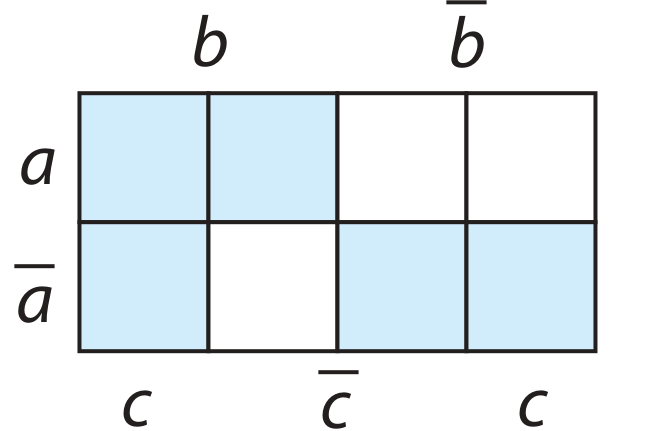
\includegraphics[width=4cm]{ex29.png}
\end{center}
\exo{}

\'Ecrire l'expression booléenne représentée par le tableau de Karnaugh suivant sous la forme d'une somme de deux variables booléennes prises parmi x, y, z, $\barmin{x}
$, $\barmin{y}$ et $\barmin{z}$.
\begin{center}
	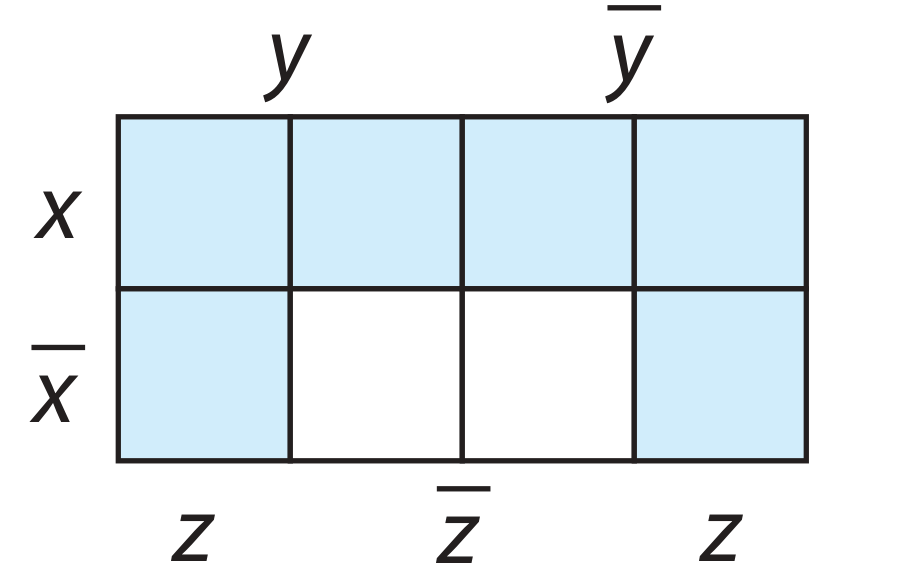
\includegraphics[width=4cm]{ex30.png}
\end{center}

\exo{}

$x$,$y$ et $z$ sont trois élément d'une algèbre booléenne B.\\

\'Ecrire l'expression $y\overline{(xy+z)}$ sous la forme d'un produit de trois variables booléennes prises parmi x, y, z, $\barmin{x}
$, $\barmin{y}$ et $\barmin{z}$.\\

\exo{}


$a$,$b$ et $c$ sont trois élément d'une algèbre booléenne B.

\begin{enumerate}[\bfseries 1.]
	\item 	\'Ecrire  l'expression $(a+\barmin{b}c)(b+\barmin{c})$ sous la forme d'une somme de deux produits de deux variables booléennes prises parmi a, b, c, $\barmin{a}
	$, $\barmin{b}$ et $\barmin{c}$.
	\item 	Représenter ce résultat dans une table de Karnaugh et en déduire une nouvelle expression\\
\end{enumerate}

\exo{}

B est une algèbre booléenne. On définit l'opération \og nor\fg{}, notée $\downarrow$ par : $$\forall a\in\mathcal{B},\forall b\in\mathcal{B},\; a\downarrow b = \overline{a+b}$$

Cette opération est dite \textit{universelle} car elle permet de retrouver toutes les autres opérations.

\begin{enumerate}[\bfseries 1.]
	\item 	Montrer que $\forall a\in\mathcal{B}\; a\downarrow a = \overline{a}$.
	\item 	En déduire que $$\forall a\in\mathcal{B},\forall b\in\mathcal{B},\; (a\downarrow b)\downarrow(a\downarrow b) = a+b$$
	\item 	Comment à partir de a, b et $\downarrow$ obtenir $ab$ ?\\
\end{enumerate}

\exo{ Polynésie juin 2018}

Une société de fabrication et d'installation de fibre optique a besoin de recruter un informaticien, femme ou homme. La direction des ressources humaines considère qu'une candidature est recevable lorsqu'elle satisfait à l'une au moins des conditions suivantes:

\begin{list}{\textbullet}{}
	\item le candidat est âgé de 25 ans ou moins et est titulaire du BTS SIO;
	\item le candidat est âgé de 25 ans ou moins, n'est pas titulaire du BTS SIO et possède de l'expérience;
	\item le candidat est âgé de strictement plus de 25 ans  et est titulaire du BTS SIO;
\end{list}

\smallskip

\begin{list}{\textbullet}{On définit les variables booléennes $a$, $b$, $c$ de la façon suivante:}
	\item $a=1$ si le candidat est âgé de strictement plus de 25 ans, $a=0$ sinon;
	\item $b=1$ si le candidat est titulaire d'un BTS SIO, $b=0$ sinon;
	\item $c=1$ si le candidat a de l'expérience, $c=0$ sinon.
\end{list}

\begin{enumerate}[\bfseries 1.]
	\item Écrire une expression booléenne $E$ traduisant qu'une candidature est recevable, à l'aide des variables booléennes $a$, $b$, $c$.
	\item À l'aide d'un tableau de Karnaugh, déterminer une écriture simplifiée de $E$ sous la forme d'une somme de deux termes. En déduire une interprétation simplifiée des conditions pour qu'une candidature soit recevable.
	\item Une candidate a 21 ans, aucune expérience, mais est titulaire du BTS SIO. Remplit-elle les critères de recrutement?
	\item Donner une expression simple de $\overline{E}$.\\
\end{enumerate}

\exo{ Polynésie mai 2017}

Cinq joueurs, notés A, B, C, D et E, jouent régulièrement à un jeu en ligne.

Chaque partie de ce jeu oppose deux adversaires.

\begin{enumerate}[\bfseries 1.]
	\item Dans cette question, on note $J = \{A, B, C, D, E\}$ l'ensemble des cinq joueurs.

	On note $V(x~;~y)$ le prédicat : \og le joueur $x$ a déjà battu le joueur $y$\fg.

	Ainsi, la valeur $V$(A ; B) est VRAI, et la valeur de $V$(B ; A) est FAUX.

	\smallskip

	On définit trois prédicats :


	\qquad \textbf{P1} : $\forall x \in J,\: \exists y \in J,\: x \neq y$  et $V(x~;~y)$

	\qquad \textbf{P2}: $\exists x \in J,\: \forall y \in J,\: x \neq y$  et $V(x~;~y)$

	\qquad \textbf{P3}: $\exists y \in J,\: \forall x \in J,\: x \neq y$  et $V(x~;~y)$

	\smallskip

	Associer à chaque prédicat P1, P2, P3, celle des trois phrases suivantes qui lui correspond parmi
	les phrases suivantes. Aucune justification n'est demandée.

	\og Il existe un joueur qui a été battu par tous les autres joueurs\fg.

	\og Tous les joueurs ont battu au moins un autre joueur \fg.

	\og Il existe un joueur qui a battu tous les autres joueurs \fg.

	\item Un joueur reçoit un bonus lorsqu'il vérifie l'un au moins des trois critères suivants:

	$\bullet~~$ le joueur a participé à 20 parties ou davantage, et il a affronté plusieurs adversaires
	différents ;

	$\bullet~~$  le joueur n'a pas affronté plusieurs adversaires différents, et il a obtenu strictement plus de
	victoires que de défaites ;

	$\bullet~~$  le joueur n'a pas obtenu strictement plus de victoires que de défaites, et il a participé à 20
	parties ou davantage.

	On définit les variables booléennes $a$, $b$, $c$ de la façon suivante:

	$a = 1$ si le joueur a participé à 20 parties ou davantage ; $a = 0$ sinon;

	$b = 1$ si le joueur a affronté plusieurs adversaires différents ; $b = 0$ sinon;

	$c = 1$ si le joueur a obtenu strictement plus de victoires que de défaites ; $c = 0$ sinon.
	\begin{enumerate}[\bfseries a.]
		\item Écrire une expression booléenne $F$ traduisant les conditions permettant à un joueur d'obtenir le bonus.
		\item À l'aide d'un tableau de Karnaugh ou d'un calcul booléen, déterminer une écriture simplifiée de $F$ sous forme d'une somme de deux termes.
		\item En déduire une formulation simplifiée des critères permettant à un joueur d'obtenir le bonus.
	\end{enumerate}
\end{enumerate}
\end{document}
